%%%%%%%%%%%%%%%%%%%%%%%%%%%%%%%%%%%%%%%%%%%%%%%%%%%%%%%%%%%%%%%%%%%%%%%%%%%%%%%%
\documentclass[twocolumn]{revtex4}
%%%%%%%%%%%%%%%%%%%%%%%%%%%%%%%%%%%%%%%%%%%%%%%%%%%%%%%%%%%%%%%%%%%%%%%%%%%%%%%%



%%%%%%%%%%%%%%%%%%%%%%%%%%%%%%%%%%%%%%%%%%%%%%%%%%%%%%%%%%%%%%%%%%%%%%%%%%%%%%%%
% Include some extra packages.
%%%%%%%%%%%%%%%%%%%%%%%%%%%%%%%%%%%%%%%%%%%%%%%%%%%%%%%%%%%%%%%%%%%%%%%%%%%%%%%%
\usepackage[]{graphicx}
%%%%%%%%%%%%%%%%%%%%%%%%%%%%%%%%%%%%%%%%%%%%%%%%%%%%%%%%%%%%%%%%%%%%%%%%%%%%%%%%



%%%%%%%%%%%%%%%%%%%%%%%%%%%%%%%%%%%%%%%%%%%%%%%%%%%%%%%%%%%%%%%%%%%%%%%%%%%%%%%%
\begin{document}
%%%%%%%%%%%%%%%%%%%%%%%%%%%%%%%%%%%%%%%%%%%%%%%%%%%%%%%%%%%%%%%%%%%%%%%%%%%%%%%%



%%%%%%%%%%%%%%%%%%%%%%%%%%%%%%%%%%%%%%%%%%%%%%%%%%%%%%%%%%%%%%%%%%%%%%%%%%%%%%%%
\title{
Final Project - Can You Escape a Velociraptor if You Get a Head Start?
}

\author{Sandy Spicer}
\affiliation{Siena College, Loudonville, NY}

\date{\today}

\begin{abstract}
    
The purpose of this project is to determine the probability of a human escaping from a velociraptor or being eaten by one. The velociraptor travels at 18 m/s while we can only travel at 3.0 m/s. Luckily, the human was given a 30 meter head start. Converting simple algebra into code to define a function, I found that the velociraptor caught up to a human in 2 seconds and after 36 meters. However, the velociraptor didn't strike until it was 1 meter away. Next, I wrote a new function that found how many seconds have passed and how far the human ran during that time. My function yielded 1.94 seconds and 34.92 meters. Finally, I calculated the probability of the `raptor biting the human when it was one meter away. I wrote another function and passed in 100 random integers, then created if and elif statements to test whether or not the human would escape. Using these statements, I created a ``for'' loop that looped over 1000 numbers and used my function to find the probability of a human escaping. The probabilities ranged from 58\% to 63\%. Overall, the odds seemed to be in our favor because this velociraptor did not prepare for the Hunger Games as well as our species. 

\end{abstract}
%%%%%%%%%%%%%%%%%%%%%%%%%%%%%%%%%%%%%%%%%%%%%%%%%%%%%%%%%%%%%%%%%%%%%%%%%%%%%%%%



%%%%%%%%%%%%%%%%%%%%%%%%%%%%%%%%%%%%%%%%%%%%%%%%%%%%%%%%%%%%%%%%%%%%%%%%%%%%%%%%
\maketitle
%%%%%%%%%%%%%%%%%%%%%%%%%%%%%%%%%%%%%%%%%%%%%%%%%%%%%%%%%%%%%%%%%%%%%%%%%%%%%%%%

%%%%%%%%%%%%%%%%%%%%%%%%%%%%%%%%%%%%%%%%%%%%%%%%%%%%%%%%%%%%%%%%%%%%%%%%%%%%%%%%
\section{Introduction}
Below, I will outline how I solved each problem. Additionally, I will explain how I figured out my code and how it works to obtain the correct answers.
%%%%%%%%%%%%%%%%%%%%%%%%%%%%%%%%%%%%%%%%%%%%%%%%%%%%%%%%%%%%%%%%%%%%%%%%%%%%%%%%


%%%%%%%%%%%%%%%%%%%%%%%%%%%%%%%%%%%%%%%%%%%%%%%%%%%%%%%%%%%%%%%%%%%%%%%%%%%%%%%%
\section{Problem 1 - Position vs. Time}

\subsection{What Was The Problem Asking?}
In Problem 1, I was given the speeds of both the velociraptor and human as well as the human's head start. I was asked to create a properly labeled position vs. time graph for the velociraptor and human that included a legend. This graph and how I coded it will be included below. 

\subsection{Python Code Explanations}
Before I wrote any code, I imported matplotlib.pylab as plt and numpy as np. By importing matplot.lib.pylab and writing ``\%matplotlib inline," I was able to plot my position vs. time graph within the notebook itself. Next, I created an empty list called time. I wrote a ``for'' loop that looped over a range of values from 0 to 500. I then defined a variable within the ``for'' loop called ``c'' and equalled it to the variable I was looping over (i) and divided by 100. I divided by 100 so that the time interval would shrink to hundredths of a second to yield more precise results. I appended the variable ``c'' to my empty list of time.

I had a very similar approach to my velociraptor and human equations. For my velociraptor equation, I created an empty list ``x1.'' Then, I used a ``for'' loop to loop over each time value that I created in the previous step. Within my ``for'' loop, I created a variable ``d'' and equalled that to 18 x i. I derived this equation by using the givens for this problem and simple algebra. I used the equation: $ \vec{v} = \frac{d}{t}.$ Since the velociraptor travels at 18 m/s, that means that it travelled 18 meters in 1 second. In order to get the velociraptor's speed for all time values, I manipulated the original equation to: $d = \vec{v}t.$ This is how I was able to get my velociraptor equation to be: $d=18i$ (i being each time value that I pass in). Next, I appended all of my distance values for the velociraptor into my empty list, x1.

I had the same exact approach for my human equation. I looped over each time value using a for loop. Next, I made an equation: $e = 3i+30.$ Since the human travels at 3 m/s, I got 3i. And because the human had a 30 meter head start, I added 30 meters to my equation. Finally, I appended my distance values into my empty list, x2.

Next, I plotted my results onto the same graph, making sure to label each plot. I made my x-label ``Time','' y-label ``Position,'' and my title ``Position vs. Time.'' I put my legend in the upper left hand corner and saved my figure to my desktop. 

\graphicspath{ {Desktop/CSIS_200_F15/} }
\begin{figure}[h]
\caption{Position vs. Time}
\footnote{Here is my Position vs. Time graph for velociraptor and human speed data.\label{fig:posvs.time}}
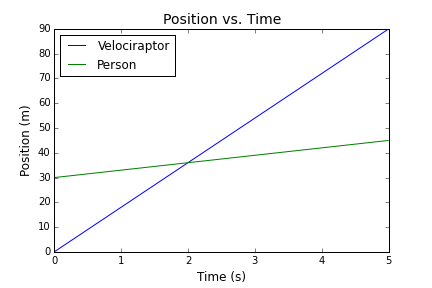
\includegraphics[width=8cm]{Position_vs_Time}
\end{figure}
%%%%%%%%%%%%%%%%%%%%%%%%%%%%%%%%%%%%%%%%%%%%%%%%%%%%%%%%%%%%%%%%%%%%%%%%%%%%%%%%


%%%%%%%%%%%%%%%%%%%%%%%%%%%%%%%%%%%%%%%%%%%%%%%%%%%%%%%%%%%%%%%%%%%%%%%%%%%%%%%%
\section{Problem 2 - When Does the `Raptor Catch Up To You?}
\subsection{What Was The Problem Asking?}
In Problem 2, I was asked to use python code to figure out how much time has passed and how far a human ran until the `raptor caught up to them.

\subsection{Python Code Explanations}
For this problem, I used algebra to create a function called, time\_and\_distance1, that passed in the velociraptor position (x1), human position (x2) as well as the time values. In order to find when the velociraptor caught up to the person and the time, I knew that you would have to set the velociraptor equation equal to the human equation, however, had to determine a way to get the same answer through coding. Within my function, I created a ``for'' loop that looped over a range of numbers from 0 to 500. Then within the ``for'' loop, I created an ``if'' statement where I implemented my knowledge of algebra. In my ``if'' statement, I said: if my velociraptor equation equals my human equation, then return my time and position values where they are equal. I used [i] because my equations are functions of time. When I returned and printed my values, I got 2 seconds and 36 meters. This means that it took the `raptor 2 seconds and 36 meters to catch up to the human, who had a 30 meter head start.

%%%%%%%%%%%%%%%%%%%%%%%%%%%%%%%%%%%%%%%%%%%%%%%%%%%%%%%%%%%%%%%%%%%%%%%%%%%%%%%%


%%%%%%%%%%%%%%%%%%%%%%%%%%%%%%%%%%%%%%%%%%%%%%%%%%%%%%%%%%%%%%%%%%%%%%%%%%%%%%%%
\section{Problem 3 - When Is It Close Enough To Strike?}
\subsection{What Was The Problem Asking?}
In Problem 3, I was asked to use python code to figure out how much time has passed and how far a human ran when the `raptor is 1 meter behind them. I was also asked to make a new copy of the plot I constructed in Problem 1, and label with an arrow the point at which the `raptor is 1 meter behind the human.

\subsection{Python Code Explanations}
For this problem, I used a similar function to the one in Problem 2. I called this function, time\_and\_distance2, that passed in the velociraptor position (x1), human position (x2) as well as the time values. Within my function, I created a ``for'' loop that looped over a range of numbers from 0 to 500. Then within the ``for'' loop, I created an ``if'' statement where I used my knowledge of algebra again. I knew that if the velociraptor equation subtracted from the human equation was less than 1, I would obtain the amount of time that has passed as well as how far the human ran. Once I returned my values t2[i] and x1[i], I found that 1.94 seconds passed by and the human ran 34.92 meters until the velociraptor was 1 meter behind.

In order to draw an arrow on my original plot, I copied all of my code from Problem 1 and added the arrow python code, which I found online. I had to play around with the parameters until the arrow was pointing at the point of intersection of the two lines. I then saved this plot to my desktop.

\graphicspath{ {Desktop/CSIS_200_F15/} }
\begin{figure}[h]
\caption{Position vs. Time Arrow}
\footnote{Here is my Position vs. Time graph for velociraptor and human speed data with an arrow labeling when the raptor is 1 meter behind the human.\label{fig:posvs.time-arrow}}
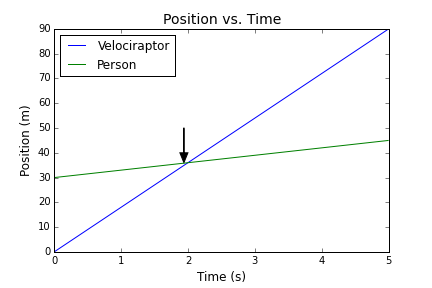
\includegraphics[width=8cm]{Position_vs_Time_Arrow}
\end{figure}

%%%%%%%%%%%%%%%%%%%%%%%%%%%%%%%%%%%%%%%%%%%%%%%%%%%%%%%%%%%%%%%%%%%%%%%%%%%%%%%%


%%%%%%%%%%%%%%%%%%%%%%%%%%%%%%%%%%%%%%%%%%%%%%%%%%%%%%%%%%%%%%%%%%%%%%%%%%%%%%%%
\section{Problem 4 - Will It Bite You?}
\subsection{What Was The Problem Asking?}
In Problem 4, I was asked to find the probability of a human escaping from a velociraptor. There is a 20\% chance that the velociraptor will bite the human on the first try. On the second try, there is a 15\% chance, and on the third try there is a 7\% chance. If the velociraptor misses after the third try, then the human escapes!

\subsection{Python Code Explanations}
First, I defined a function called ``bite''. Within the function, I created three separate equations for each bite. I set each equation equal to 100 random integers. Next, I used if, elif, and else statements within my function. If the first try was less than or equal to 20, then I had the function return that the velociraptor has bitten you. If the second try was less than or equal to 15, then the velociraptor also bit you. And if the third try was less than or equal to 7, the function returned that the velociraptor has bitten you. Finally, I used an else statement that returned: You will escape. If all of the previous ``if'' statements were false, meaning that the velociraptor failed to bite the human, then that means that the human must have escaped. Next, I assigned two variables with the starting value of 0. These variables were failures and successes. Then, I did a ``for'' loop that looped over a range of numbers from 0 to 1000. Within the ``for'' loop, I made ``i,'' the number I was passing in, go up by one each time. I set my bite function equal to a variable, called t. Then I wrote if and elif statements. I said: if my bite function equalled, ``The velociraptor has bitten you.'', then add one to failures. Otherwise, if my bite function was equal to: ``You will escape!", then it added one to successes. After this, I wrote an equation for probability and set it equal to the amount of successes (or how many times the human escaped) divided by 1000. In order to get a percentage as my answer, I multiplied the equation by 100. Since I used random numbers to generate my probability, I got a different answer each time. However, the percentages ranged from 58\% all the way to a little over 63\%.

%%%%%%%%%%%%%%%%%%%%%%%%%%%%%%%%%%%%%%%%%%%%%%%%%%%%%%%%%%%%%%%%%%%%%%%%%%%%%%%%


%%%%%%%%%%%%%%%%%%%%%%%%%%%%%%%%%%%%%%%%%%%%%%%%%%%%%%%%%%%%%%%%%%%%%%%%%%%%%%%%
\section{Conclusion}

Overall, it is more likely than not to escape from a velociraptor if you have a head start. This project tested my ability to convert algebra into code as well as incorporated nearly every topic that we have covered in this class from the beginning. I had to use loops, functions, plotting, and conditionals in addition to my physics knowledge. This assignment was quite challenging, but an exciting one that forced me to critically think and design my own code. 

%%%%%%%%%%%%%%%%%%%%%%%%%%%%%%%%%%%%%%%%%%%%%%%%%%%%%%%%%%%%%%%%%%%%%%%%%%%%%%%%
\end{document}
%%%%%%%%%%%%%%%%%%%%%%%%%%%%%%%%%%%%%%%%%%%%%%%%%%%%%%%%%%%%%%%%%%%%%%%%%%%%%%%%
